\section{Reinforcement Learning (RL)}\label{sec:rl}
  One of the tried and tested methods of end-to-end learning approaches is a branch under machine learning called \emph{Reinforcement Learning (RL)}. 

  \begin{figure}[h]
    \centering
    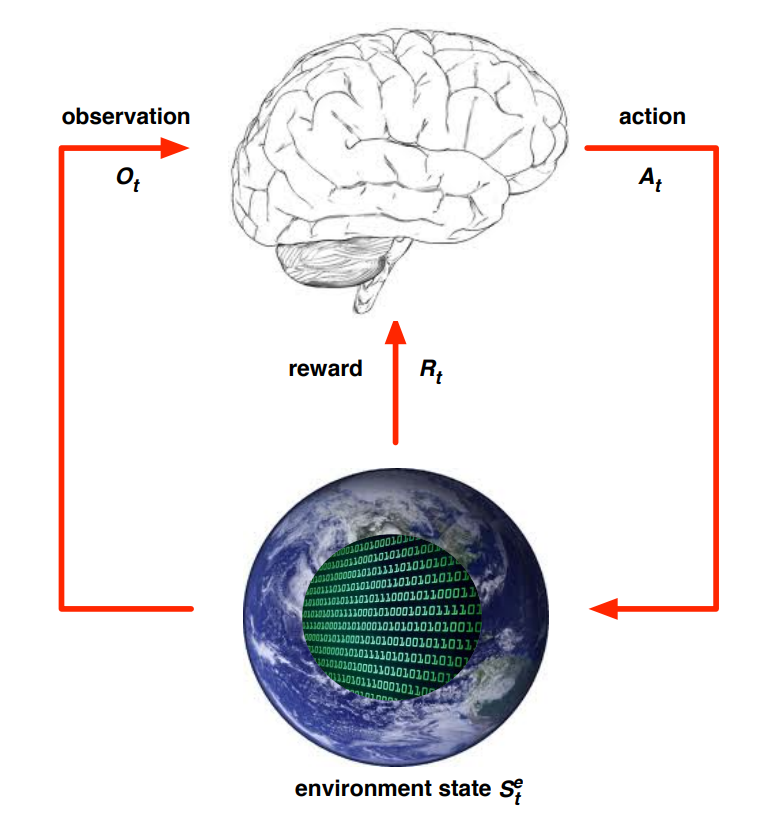
\includegraphics[width=0.3\linewidth]{assets/background/silver-rl.png}
    \caption{Simple RL diagram to reinforce intuition \cite{silver2015}}\label{fig:rl-diag}
  \end{figure}

  RL's main focus is training algorithms, which are called \emph{agents}, in making optimal decisions by interacting with the environment. The key objective is to teach a \emph{policy} to the agent that maximises the overall reward -either internally defined or externally provided by a \emph{teacher}. The agent will explore the possible actions it can take through trial and error, while learning from the feedback given to it by the reward signal and its environment.One of the differentiating factors of RL from classical machine learning paradigms is that the feedback is not instantaneous and sequences of decisions influence the subsequent data and signals given to agent \cite{silver2015}.

\subsection{RL in Practice}
  Reinforcement learning, can be used to train a variety of agents that is not limited by physical robots. It can learn to play video-games \cite{comi2018}, automation tasks, in natural language processing \cite{paulus2017deepreinforcedmodelabstractive}, applications in healthcare (where RL is categorised as dynamic treatment regimes) for use in chronic diseases or critical care \cite{yu2020reinforcementlearninghealthcaresurvey} and lastly learning movement behaviours for robots.

  \subsection{Exploration and Exploitation}
  
  A fundamental challenge in utilising RL is the constant act of balancing \textbf{exploration} and \textbf{exploration}. A trade-off must be made in the created system.
  \begin{enumerate}
    \item \textbf{Exploration:}
    This is when the agent decides to \emph{explore} new actions that might potentially lead to better long-term outcomes. An issue this can cause is that the time it takes to explore all possibilities might not be feasible. But crucial to utilise in in problems with sparse reward models.\todo[color=green]{citations}.
    \item \textbf{Exploitation:}
    When the agent prioritises short-term, immediate rewards by exploiting its current knowledge. For example, taking an agent playing a video game; if a high score was found the agent might be unaware that a higher score can be achieved with a different set of moves. 
  \end{enumerate}
  
  Sampling efficiencies and ease of training \cite{liu2019simpleexplorationsampleefficient} should also be considered with each,. To relate it back to a robotics example, too much exploration might lead to  inefficient training and instability; while too much reliance on exploitation might lead to suboptimal behaviours in the movement of a robot executing a task. Along with this widespread use and elemental challenges, comes differing methods of utilising the RL framework. The likes of which can be broadly classified into two types: 

  \subsubsection{Model-Based RL}
  Involves creating an internal model of the state the agent is within. Involves a dynamics model, then planning within it \cite{MAL-086}. They usually have underlying principals of MDPs (\ref{sec:mdp}). This helps to learn in a simulated mode. Fewer real interactions allows sample efficiencies \cite{liu2021DRLminireview,wu23robotLearn}, meaning amount of time spent to learn optimal policies are quite low. Knowing the model also removes the guess work of unknown states and hence generalisation is easier for unknown states \cite{MAL-086}.

  However, there are negatives. The model introduces a bias which leads inadequate representations or faulty models to learn policies  that exploit these deficiencies \cite{Deisenroth2011PILCO,wang2019benchmarkingmodelbasedreinforcementlearning}. Some recent works have characterised the uncertainty and alleviated that bias \cite{kurutach2018modelensembletrustregionpolicyoptimization, chua2018deepreinforcementlearninghandful, clavera2018modelbasedreinforcementlearningmetapolicy}. Also coupling the model and the policy learning which makes agents more prone to performance local-minima, which stems from exploitation not being fully investigated in these settings. Some applications are motion planning, trajectory optimisation and learning from limited interactions, some common methods are: Monte Carlo Tree Search (MCTS),Probabilistic Inference for Learning Control (PILCO) \cite{Deisenroth2011PILCO}, MuZero: Combines model-based approaches with deep learning.\todo[color=green]{cite here}

  \subsubsection{Model-Free RL}
  This collection of schemes attempt to learn a policy directly by trial and error, without explicitly modelling the environments dynamics. Usually preferred when the environment is too complex or too costly to model. There are a few different variants of model-free approaches, all of them similar in the way they omit a model, but have different methods in extracting the optimal policies.
  \begin{itemize}
    \item \textbf{Value-Based:} Learn from value of states (or an estimate) and actions. They learn $v_\pi$ $q_\pi$ to then extract the optimal policy, $\pi_*$. Mainly used for simple navigation, basic motor and arm control.Q-Learning [Off-Policy], Deep Q-Networks (DQN) [Off-Policy], SARSA [On-Policy]. \todo[color=green]{citations}
    \item \textbf{Policy-Based} Learn the policy directly, bypassing values, stattes or actions completely. Helpful when the state-space is large. For example, for infinite spaces, value-based approaches are impossible.Used for complex control tasks, such as dexterous limb manipulation, robot hand grasping. Some examples are: REINFORCE [On-Policy], Proximal Policy Optimisation (PRO) [On-Policy], Trust Region Policy Optimisation (TRPO) [On-Policy]. \todo[color=green]{citations}
    \item \textbf{Actor-Teacher} Policy is improved from direct feedback coming from a \emph{teacher}. Which can be an external system or an ``expert human'' providing demonstrations (see \ref{sec:il}).Some common approaches are
      \begin{itemize}
        \item \textbf{Direct Action Supervision}: where the teacher suggest actions directly to the agent.
        \item \textbf{Criticising Actions}: where the actions are suggested by the teacher.\todo{not sure if this makes sense}
        \item \textbf{Shaped Rewards}: the teacher modifies the reward signal dynamically to encourage desirable behaviours.
        \item \textbf{Curriculum Learning}: the teacher controls the difficulty of tasks over time to ease the learning of the agent.
      \end{itemize}
  \end{itemize}
  
  Mixing the two together is also a viability for some hybrid approaches. Characteristics from each can be combined to merge their benefit from different guarantees each provides \cite{qu2020combiningmodelbasedmodelfreemethods}
  On top of the model dependence, the RL approach can be of two flavours:

  \subsection{On-Policy}
  This approach means that the agent updates its policy from data generated by the current policy. So an agent can only learn from the actions it purposefully took under its latest policy. Which can restrict improvements, but means that no outdated or stale data can influence the present time actions or learning.
  This leads to more stable learning in stochastic environments \todo[color=green]{citation?} while ensuring policy consistency.

  However, it also means that the agent becomes sample inefficient, as fresh iterations are needed to learn and sharpen the current policy. On top of that, the learning rate slows down because the agent can't use older experience (only the latest policy), slowing training \cite{andrychowicz2020onpolicyRL}.

  \subsection{Off-Policy}
  In this case, the agent can utilise past experiences, regardless of the policy generated by the training. This recycling of information previously known makes the learning more efficient \cite{uehara2022reviewoffpolicyevaluationreinforcement}, as sample efficiency is increased.
  Having past experiences also means that the agent will need fewer exploration steps and less iterations because of these priors.
  
  This however, brings instability in stochastic environments, and the the policy diverging due to incorporating outdated and possibly uninformative data (at least currently). Therefore, some sort of importance of older steps should be kept track of, and maybe even decayed like the discount factor from MDPs (\ref{sec:mdp}). \cite{maroti2019rbed} 
  \\\\
  Both of these approaches can be combined with either \textbf{Model-Based} or \textbf{Model-Free} approaches. Because at the end of the day, making a good model is about picking the correct trade-offs that is relevant to the scenario of the problem we are attempting to solve.
